\documentclass{scrbook}
\usepackage{graphicx} % Required for inserting images
\usepackage{tabularx} % Required for fixed width tables
\usepackage{scrlayer-scrpage} % Required for the subtitles
\usepackage{url} % Required for the URLs
\usepackage{hyperref} % Required for the URLs
\usepackage{listings} % Required for the code snippets
\usepackage{mathtools} % Required for the system of equations
\usepackage{amsmath,amssymb} % Required for some math symbols
\usepackage{enumitem} % Required for lettered lists

% Put the caption of the snippets at the bottom
\lstset{
    captionpos=b
}


\title{Web accessibility}
\subtitle{Ambient intelligence course (A.Y. 2025/2026)\\Topic taught by Prof. Floriano Scioscia}
\author{Gabriele Colapinto}
\date{\today}

\begin{document}

\maketitle
\thispagestyle{empty}

{\Large\textbf{License}} \\
{Notes from Ambient intelligence (A.Y. 2025/2026) by Gabriele Colapinto. 
Course taught by professors Michele Ruta, Floriano Scioscia, Arnaldo Tomasino, Davide Loconte — 
Licensed under CC BY-NC 4.0.\\
\url{https://creativecommons.org/licenses/by-nc/4.0/}}

\vspace*{\fill}
\rule{\textwidth}{0.2pt}
\small{© 2025 Gabriele Colapinto \\
Released under the \href{https://creativecommons.org/licenses/by-nc/4.0/}{Creative Commons Attribution–NonCommercial 4.0 International License}}

\clearpage

\tableofcontents

\chapter{Defining the Core Concepts of Accessibility}

To engage in a meaningful discussion about creating inclusive digital environments, we must first establish a shared vocabulary. The terms 'disability,' 'accessibility,' and 'assistive technology' are not mere jargon; they represent foundational concepts that shape our entire approach to web design and development. A clear, mutual understanding of these core principles is the necessary groundwork upon which all effective accessibility practices are built.

\section{The Principle of Web Accessibility}

The core vision of web accessibility is intertwined with the very purpose of the World Wide Web itself. As its inventor, Tim Berners-Lee, stated, “The power of the Web is in its universality. Access by everyone regardless of disability is an essential aspect.”. Web accessibility is the practical fulfillment of that vision. A web cannot be truly universal if it excludes a significant portion of the population. The practice of accessibility, therefore, is the work of ensuring that the web is for everyone, transforming its universal potential into a tangible reality.

\section{Defining Disability: From Personal Trait to Environmental Mismatch}

Our modern understanding of disability has undergone a significant paradigm shift from earlier models. The current global standard is the "Bio-Psycho-Social model", formally articulated in the \textbf{United Nations Convention on the Rights of Persons with Disabilities (2006)}. This framework defines disability not as an inherent personal trait but as a contextual phenomenon.


\begin{quote}
“Recognizing that disability is an evolving concept and that disability results from the interaction between persons with impairments and attitudinal and environmental barriers that hinders their full and effective participation in society on an equal basis with others”

— \textit{United Nations Convention on the Rights of Persons with Disabilities, 2006}
\end{quote}

This definition marks a crucial departure from the perspectives of the 1960s, which often framed disability as an "ethical" or intrinsic feature of a person. The modern model reframes the issue entirely: disability is understood as the negative outcome of an \textit{interaction}. It arises when a person with a functional impairment encounters environmental or attitudinal barriers that prevent their equal participation in society. The problem is not the person's impairment, but the mismatch between their needs and the environment.

\section{Defining Accessibility: Proactive Inclusion}

If disability is the result of barriers, then accessibility is the proactive solution to eliminating them. It is the practice of designing environments, products, and services that prevent these disabling mismatches from occurring. The \textbf{United Nations Convention} defines accessibility as ensuring "access, on an equal basis with others, to the physical environment, to transportation, to information and communications, including information and communications technologies and systems". \\

The \textbf{ISO/IEC 30071-1:2019 standard} provides a more technical definition, describing accessibility as the "extent to which products, systems, services, environments and facilities can be used by people from a population with the widest range of user needs, characteristics and capabilities". \\

Synthesizing these definitions, accessibility is the measure of how inclusively a product or system is designed. It aims for maximum usability by the widest possible range of people, accommodating their diverse capabilities either directly or through the support of assistive technologies.

\section{Defining Assistive Technology: Tools for the Individual}

While closely related to accessibility, assistive technology represents a different, though complementary, perspective. The \textbf{ISO/IEC 30071-1:2019} specification defines it as "hardware or software that is added to or incorporated within an ICT system that increases accessibility for an individual". It is a tool tailored to a specific person to help them overcome barriers.

The distinction between the two concepts is best understood by their starting points:

\begin{itemize}
    \item \textbf{Accessibility:} Starts from the perspective of the service, tool, or environment. Its goal is to be maximally usable for \textit{everyone}.
    \item \textbf{Assistive Technology:} Starts from the perspective of the \textit{individual}. It provides tailored tools that help a specific person access an environment or service.
\end{itemize}

Common examples of assistive technologies range from the everyday, such as \textbf{glasses}, to highly specialized digital tools like \textbf{screen readers for blind people} (figure ~\ref{fig:screen_reader}) or \textbf{eye trackers for individuals with motor impairments} (figure ~\ref{fig:eye_tracker}) who cannot use a traditional keyboard or mouse.

\begin{figure}
    \centering
    
\includegraphics[width=\linewidth]{Images/Screen_reader.jpg}
    \caption{Screen reader}
    \label{fig:screen_reader}
\end{figure}

\begin{figure}
    \centering
    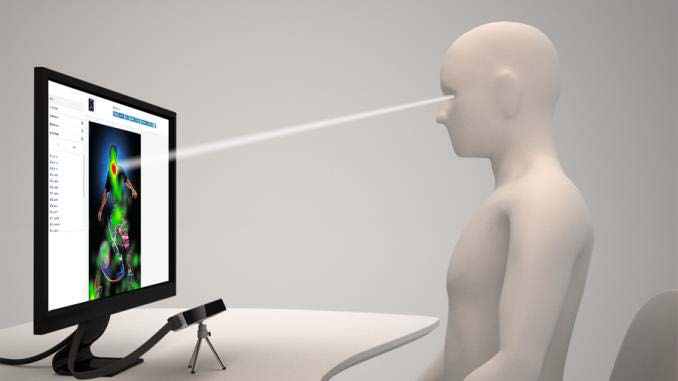
\includegraphics[width=\linewidth]{Images/Eye_tracker.jpg}
    \caption{Eye tracker}
    \label{fig:eye_tracker}
\end{figure}

With these foundational concepts defined, we can now explore the historical evolution of the design philosophies that put these ideas into practice.

\chapter{The Evolution of Accessible Design Philosophies}

Current best practices in accessible design are not a recent invention but the culmination of decades of progressive thought. This evolution reflects a significant shift in perspective, moving away from a reactive model of regulatory compliance toward a proactive philosophy of inclusive, human-centered design from the outset.

\section{Barrier-Free Design: The Regulatory Approach}

The "Barrier-free design" philosophy emerged in the United States during the 1960s, with a primary perspective of meeting legal regulations. Its origins are linked to the American Civil Rights Movement, which, in its pursuit of equality for all citizens, began to consider disability-based inequality alongside racial inequality. This approach led to landmark legislation, including the \textbf{U.S. Civil Rights Act (1964)} and the \textbf{Americans with Disabilities Act (1990)}, which mandated the removal of barriers in physical and, eventually, digital spaces.

\section{Universal Design: A Paradigm Shift}

A significant conceptual leap occurred with the introduction of "Universal Design," a term coined by \textbf{Ronald L. Mace} and a philosophy advanced by contemporaries like \textbf{Selwyn Goldsmith}, who popularized key examples of its principles. This philosophy represented a fundamental shift away from designing for a hypothetical "standard person"—an able-bodied, right-handed individual—and toward considering the needs of all potential users simultaneously.


The classic example illustrating this principle is the \textbf{curb ramp} (figure ~\ref{fig:curb_ramp}). While designed to provide access for wheelchair users, it offers significant benefits to parents with strollers, travelers with wheeled luggage, and delivery workers, all without decreasing usability for anyone else. This highlights a core tenet of Universal Design: features that improve accessibility for one group should not create new barriers for others and, ideally, should benefit a wide range of users.

\begin{figure}
    \centering
    
\includegraphics[width=0.5\linewidth]{Images/Curb_ramp.jpg}
    \caption{Curb ramp}
    \label{fig:curb_ramp}
\end{figure}

\section{Design for All: The European Counterpart}

In Europe, a parallel school of thought known as "Design for All" developed, beginning in Sweden in the 1970s. Sharing the same fundamental principles as Universal Design, this movement focuses on creating products and environments that are accessible to the widest possible audience. The \textbf{EIDD Stockholm Declaration (2004)} stands as a landmark moment for this movement, formally articulating its goal as "Design for human diversity, social inclusion and equality".

\section{The Seven Principles of Universal Design}

The philosophy of Universal Design is guided by seven core principles that provide a framework for creating broadly inclusive designs:

\begin{enumerate}
    \item \textbf{Equitable use}
    \item \textbf{Flexibility in use}
    \item \textbf{Simple and intuitive}
    \item \textbf{Perceptible information}
    \item \textbf{Tolerance for error}
    \item \textbf{Low physical effort}
    \item \textbf{Size and space for approach and use}
\end{enumerate}

These broad philosophies provide the ethical and practical foundation for accessibility. We now turn to how they have been specifically applied to the domain of Information and Communications Technology (ICT) and the World Wide Web.

\chapter{Web Accessibility in Practice: The W3C and Legal Frameworks}

The abstract principles of universal design have been formally adapted, codified, and mandated for the digital realm. This process has been driven by both international standards bodies, which define the technical "how", and legislative frameworks, which provide the legal "why". This section explores the key organization driving these standards—the W3C's Web Accessibility Initiative (WAI)—and the legal mandates that require their implementation.

\section{The W3C Web Accessibility Initiative (WAI)}

The \textbf{WAI} is a permanent working group within the World Wide Web Consortium (W3C), the main international standards organization for the Web. Its mission is to ensure that W3C technologies, particularly the web, serve the needs of people with disabilities. This mission has two equally important goals:

\begin{itemize}
    \item To enable people with disabilities to perceive, understand, navigate, and interact with the Web.
    \item To empower people with disabilities to \textit{contribute} to the Web, ensuring they can be creators and producers of content, not just consumers.
\end{itemize}

\section{The Broad Spectrum of Inclusion and Its Benefits}

The WAI's work addresses a wide range of functional impairments to ensure comprehensive inclusion. These categories include:

\begin{itemize}
    \item Visual
    \item Auditory
    \item Speech
    \item Physical
    \item Neurological
    \item Cognitive
\end{itemize}

Adopting this inclusive approach yields significant "side benefits" that improve the usability of a website or application for all users in various contexts. Designing for these impairments creates a more robust and flexible user experience for:

\begin{itemize}
    \item Users of mobile phones, smart watches, and other devices with small screens or different input modes.
    \item Older people experiencing changing abilities due to aging.
    \item People with temporary disabilities, such as a broken arm.
    \item People with situational limitations, such as being in a bright, sunny environment or a place where they cannot listen to audio.
    \item Users with a slow or limited internet connection.
\end{itemize}

\section{Key Legislative Frameworks for ICT Accessibility}

Alongside technical standards, a growing body of law mandates digital accessibility. These legal frameworks make accessibility a requirement, not just a recommendation.

\begin{itemize}
    \item \textbf{US Rehabilitation Act ("Section 508"), 1998:} The first law dedicated to accessibility in ICT.
    \item \textbf{Italian Law 4/2004 ("Legge Stanca"):} The first Italian law concerning ICT accessibility.
    \item \textbf{EU Directive 2102/2016:} Mandates accessibility for the web and mobile applications of public agencies. This was later extended to require large private corporations to meet the same standards, while smaller entities may have fewer mandatory requirements.
\end{itemize}

These standards and laws define what must be achieved. The final step is understanding the interconnected system of components that work together to make it happen.

\chapter{The Ecosystem of Web Accessibility}

\begin{figure}
    \centering
    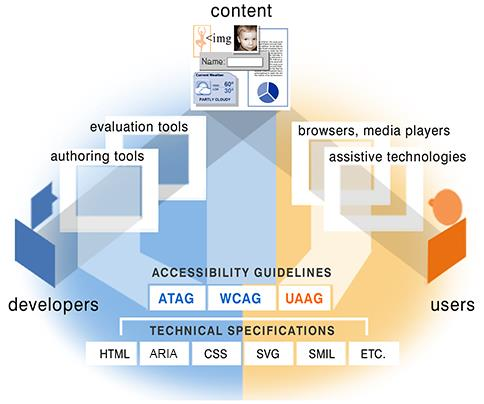
\includegraphics[width=\linewidth]{Images/Web_accessibility_ecosystem.jpg}
    \caption{Web accessibility ecosystem}
    \label{fig:web_accessibility_ecosystem}
\end{figure}

Web accessibility is not the result of a single action or the responsibility of a single group. It is the product of a complex and interdependent ecosystem where developers, tools, technologies, and users must all work in concert (See figure ~\ref{fig:web_accessibility_ecosystem}). A failure in one part of this system can undermine the entire effort. This section deconstructs this system into its core components and examines the dynamic cycle that either promotes or hinders widespread accessibility.

\section{The Core Components}

The web accessibility ecosystem is comprised of several essential, interrelated components:

\begin{itemize}
    \item \textbf{Content:} The information on a webpage or application, including text, images, and sounds, as well as the underlying code and markup that defines its structure.
    \item \textbf{User Agents:} The software that retrieves and presents web content to users, such as web browsers, media players, and streaming applications.
    \item \textbf{Assistive Technology:} The hardware and software tools, like screen readers or alternative keyboards, that users with disabilities employ to interact with user agents and content.
    \item \textbf{Users:} The people using the web, whose knowledge, experiences, and adaptive strategies are a critical part of the equation.
    \item \textbf{Developers:} The full range of people who create web content, including designers, coders, authors, and users who contribute content.
    \item \textbf{Authoring Tools:} The software—such as content management systems or code editors—used by developers to create websites and content.
    \item \textbf{Evaluation Tools:} The software and validators used to assess the accessibility of web content, such as HTML and CSS validators.
\end{itemize}

\section{The Implementation Cycle: A Virtuous System}

When all components of the ecosystem work in harmony, they create a positive feedback loop known as the "Implementation Cycle" (See figure ~\ref{fig:implementation_cycle}). This creates a virtuous cycle where accessibility support in one component, such as browsers and assistive technologies, incentivizes developers to implement corresponding features. In turn, widespread developer demand pushes authoring tools to make implementation seamless, leading to a greater volume of accessible content. This increase in accessible content empowers users with disabilities, who then expect and advocate for even broader support, creating a self-reinforcing loop that drives accessibility forward.

\begin{figure}
    \centering
    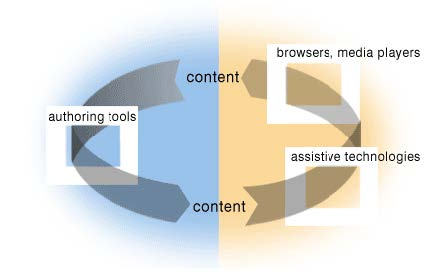
\includegraphics[width=0.5\linewidth]{Images/Implementation_cycle.jpg}
    \caption{Implementation cycle}
    \label{fig:implementation_cycle}
\end{figure}

\section{Breaking the Cycle: The Consequences of Failure}

This implementation cycle is fragile. If one component fails to provide adequate accessibility support, it breaks the chain and removes the motivation for others to act, as their efforts alone will not result in a fully accessible user experience. When the cycle is broken, stakeholders are often forced into difficult and inefficient workarounds:

\begin{itemize}
    \item \textbf{Developers} must expend extra effort to compensate for poor authoring tools, for example by coding markup directly instead of relying on the tool.
    \item \textbf{Users} must expend extra effort to compensate for inaccessible content or tools, for example by using multiple different browsers or assistive technologies to overcome specific issues.
\end{itemize}

In most cases, these workarounds are not implemented due to the high effort required. A broken cycle ultimately leads to poor accessibility or, for some users, complete inaccessibility, defeating the web's promise of universality.

\chapter{Introduction to the Web Accessibility Initiative (WAI) Framework}

The World Wide Web Consortium (W3C) established the Web Accessibility Initiative (WAI) as the central, authoritative body for creating the international standards that ensure digital accessibility. The strategic importance of this initiative lies in providing a structured and comprehensive framework that guides developers, designers, and organizations in creating digital content that is accessible to all users, including those with disabilities. By defining clear specifications, the WAI ensures a consistent and reliable approach to building an inclusive web.

The WAI framework is built upon four essential specifications, each targeting a different component of the digital ecosystem:

\begin{itemize}
    \item \textbf{Authoring Tool Accessibility Guidelines (ATAG):} These guidelines are for the creators of software that people use to build web content, such as content management systems and code editors. They ensure that these development tools are themselves accessible to developers with disabilities and that they help produce accessible content.
    \item \textbf{Web Content Accessibility Guidelines (WCAG):} This is the core standard for web content itself. It is used by developers, authoring tools, and accessibility evaluation tools to ensure that websites, applications, and other digital content are accessible.
    \item \textbf{User Agent Accessibility Guidelines (UAAG):} These guidelines target web browsers, media players, and other "user agents" that render web content. They ensure this software works effectively with assistive technologies to provide an accessible user experience.
    \item \textbf{Accessible Rich Internet Applications (ARIA):} This suite is a technical specification for making dynamic content and advanced user interface controls in modern web applications accessible.
\end{itemize}

Among these pillars, the Web Content Accessibility Guidelines (WCAG) serve as the foundational standard for the content that users ultimately interact with, and thus warrant a deeper examination.

\chapter{The Core Standard: Web Content Accessibility Guidelines (WCAG)}

The Web Content Accessibility Guidelines (WCAG) are the most widely recognized and adopted standard for web content accessibility globally. First defined in 1999, WCAG has evolved to keep pace with changing technologies. The most recent version, WCAG 2.2, was finalized in 2023, and work is currently underway on the next major iteration, version 3.0, which is in the working draft stage. WCAG provides a detailed, technical framework for making web content accessible. \\

The architecture of WCAG is hierarchical, designed to translate high-level concepts into concrete, testable requirements (See figure ~\ref{fig:wcag_architecture}). This structure is organized into three distinct levels:

\begin{itemize}
    \item \textbf{Level 1, 4 Principles:} At the highest level are four guiding principles that form the foundation of web accessibility: Perceivable, Operable, Understandable, and Robust.
    \item \textbf{Level 2, 13 Guidelines:} Each principle is expressed through one or more guidelines. These 13 guidelines provide the basic goals that authors should work toward to make content more accessible to users with different disabilities.
    \item \textbf{Level 3, Testable Success Criteria:} For each guideline, there are specific, measurable rules that can be objectively verified. They are categorized into three levels of conformance:
    \begin{itemize}
        \item \textbf{Level A:} The most essential, basic accessibility requirements.
        \item \textbf{Level AA:} Intermediate requirements that address the most common barriers for disabled users. This level is the most common target for legal and policy compliance because of its broad impact.
        \item \textbf{Level AAA:} The most advanced and comprehensive accessibility requirements.
    \end{itemize}
\end{itemize}

\begin{figure}
    \centering
    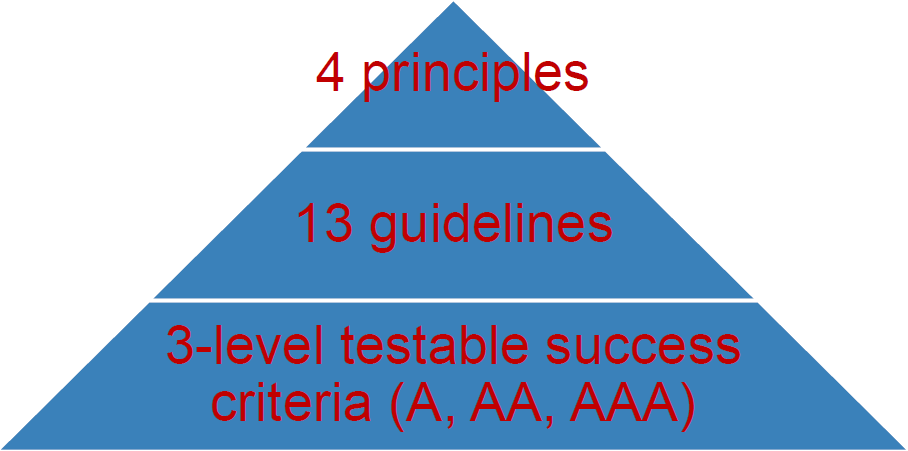
\includegraphics[width=0.5\linewidth]{Images/WCAG_architecture.png}
    \caption{WCAG architecture}
    \label{fig:wcag_architecture}
\end{figure}

\section{Principle 1: Perceivable}

The \textbf{Perceivable} principle requires that information and user interface components must be presentable to users in ways they can perceive. This means that content cannot be invisible to all of a user's senses; every user must be able to perceive the information being presented, regardless of their sensory abilities. \\

\subsection{Text Alternatives} 
All non-text content, such as images, must have a text alternative that serves the equivalent purpose. This allows assistive technologies like screen readers to convey the meaning of the content to users.

\paragraph{Exceptions}
Text alternatives are not strictly required for certain types of content, including input controls, time-based media, tests, purely sensory experiences (like art), CAPTCHAs, and content that is purely decorative.


\subsection{Time-based Media}
Alternatives must be provided for both pre-recorded and live time-based media (audio and video). This ensures that users with auditory or visual impairments can access the information.

\paragraph{Requirements}
Success criteria define various combinations of alternatives, which can include captions for audio content, audio descriptions for video content, sign language interpretation, and equivalent information (such as a transcript or summary).

\subsection{Adaptable}
Content must be created so that it can be presented in different ways—for example, in a simpler layout—without losing information or its underlying structure.

\paragraph{Requirements}
\begin{itemize}
    \item The structure of the page, the relationships between its parts, and the correct reading sequence must be programmatically determinable by user agents and assistive technologies.
    \item Instructions for understanding or operating content must not rely solely on sensory characteristics such as shape, color, size, visual location, or orientation.
    \item Content must not restrict its view and operation to a single display orientation (e.g., portrait or landscape).
    \item The purpose of each input field collecting user information, as well as the purpose of UI components, icons, and regions, must be programmatically determinable.
\end{itemize}

\subsection{Distinguishable}
Content must be designed to make it easy for users to see and hear by separating the foreground from the background.

\paragraph{Requirements}
\begin{itemize}
    \item Color must not be used as the only means of conveying information.
    \item Text and images of text must have a high contrast ratio against their background.
    \item Text must be resizable without loss of content or functionality.
    \item Pre-recorded audio should have minimal or no background noise to ensure clarity.
    \item Content must be able to reflow (e.g., into a single column) without loss of information and without requiring two-dimensional scrolling.
    \item Minimum text spacing specifications must be met to ensure readability.
    \item Content that appears on hover or focus (like a tooltip) must be dismissible, hoverable, and persistent until the user dismisses it.
\end{itemize}

\section{Principle 2: Operable}

The \textbf{Operable} principle dictates that user interface components and navigation must be operable. The interface cannot require an interaction that a user is physically unable to perform.

\subsection{Keyboard Accessible}
All functionality of the content must be operable through a keyboard interface without requiring specific timings for individual keystrokes. This is critical for users who cannot use a mouse or other pointer-based devices.

\paragraph{Requirements}
\begin{itemize}
    \item Focus must be movable to and from all interactive components using only the keyboard.
    \item Keyboard shortcuts must be able to be turned off or remapped to avoid conflicts with assistive technology commands.
\end{itemize}

\subsection{Enough Time}
Users must be provided with enough time to read and use the content.

\paragraph{Requirements}
\begin{itemize}
    \item For any time limits, there must be a mechanism to pause, stop, or extend the time.
    \item For content that moves, blinks, or auto-updates, users must be able to pause or stop it.
    \item If an authenticated session expires, user data from that activity should not be lost upon re-authentication.
\end{itemize}

\subsection{Seizures and Physical Reactions}
Content must be designed in a way that does not cause seizures or other adverse physical reactions.

\paragraph{Requirements}
\begin{itemize}
    \item Web pages must not contain anything that flashes more than three times in any one-second period.
    \item Motion animation triggered by user interaction should be disable-able unless it is essential to the functionality.
\end{itemize}

\subsection{Navigable}
The design must provide ways to help users navigate, find content, and determine their current location within a site or application.

\paragraph{Requirements}
\begin{itemize}
    \item A mechanism must be available to bypass blocks of content that are repeated on multiple pages (e.g., a "skip to main content" link).
    \item Provide descriptive page titles, headings, and labels.
    \item Ensure that components receive focus in a logical and meaningful order.
    \item The keyboard focus indicator must always be visible.
    \item Offer more than one way to locate a web page within a set of pages.
\end{itemize}

\subsection{Input Modalities}
It should be easy for users to operate functionality through various inputs beyond the standard keyboard.

\paragraph{Requirements}
\begin{itemize}
    \item Complex gestures (like multi-point or path-based gestures) should have simpler alternatives.
    \item The target size for pointer inputs (like buttons) must be large enough to be easily activated.
\end{itemize}

\section{Principle 3: Understandable}

The \textbf{Understandable} principle states that users must be able to understand the information as well as the operation of the user interface. The content or its operation cannot be beyond their comprehension. The general benchmark for readability is a level not more advanced than a lower secondary education (i.e., a junior high school student).

\subsection{Readable}
Text content must be readable and understandable.

\paragraph{Requirements}
\begin{itemize}
    \item The primary human language of the page must be programmatically determinable.
    \item A mechanism should be available for identifying the definitions of unusual words or phrases, the expanded form of abbreviations, and the specific pronunciation of words where meaning is ambiguous.
\end{itemize}

\subsection{Predictable}
Web pages should appear and operate in predictable ways, building user confidence and reducing cognitive load.

\paragraph{Requirements}
\begin{itemize}
    \item Navigational mechanisms that are repeated across multiple pages should be consistent.
    \item Unexpected changes of context (e.g., opening a new window) should be avoided. Any changes of context should be initiated by user request, or if they happen automatically (like a news ticker), they must do so in a predictable way that is easy to understand.
\end{itemize}

\subsection{Input Assistance}
Users should be helped to avoid and correct mistakes.

\paragraph{Requirements}
\begin{itemize}
    \item Input errors must be identified and described to the user in text.
    \item Clear labels and instructions must be provided for any content requiring user input.
    \item For pages involving legal or financial transactions, users must be given the opportunity to review, confirm, and correct information before final submission.
\end{itemize}

\section{Principle 4: Robust}

The \textbf{Robust} principle requires that content must be robust enough that it can be interpreted reliably by a wide variety of current and future user agents, including assistive technologies. As technology evolves, the content should remain accessible.

\subsection{Compatible}
Compatibility with current and future user agents must be maximized. This ensures that assistive technologies can accurately interpret and parse content.

\paragraph{Requirements}
\begin{itemize}
    \item Content implemented using markup languages must be well-formed, with complete start and end tags, correct element nesting, no duplicate attributes, and unique IDs.
    \item For all user interface components, their name and role must be programmatically determinable.
    \item States, properties, and values that can be set by the user must be programmatically settable.
    \item Notification of any changes to these states and properties must be available to user agents and assistive technologies.
    \item Status messages must be programmatically determinable so they can be presented to the user by assistive technologies without receiving focus.
\end{itemize}

By adhering to these four principles, WCAG provides a comprehensive framework for creating accessible web content. However, for this content to be truly accessible, the software that renders it and the tools used to create it must also follow established standards.

\begin{figure}
    \centering
    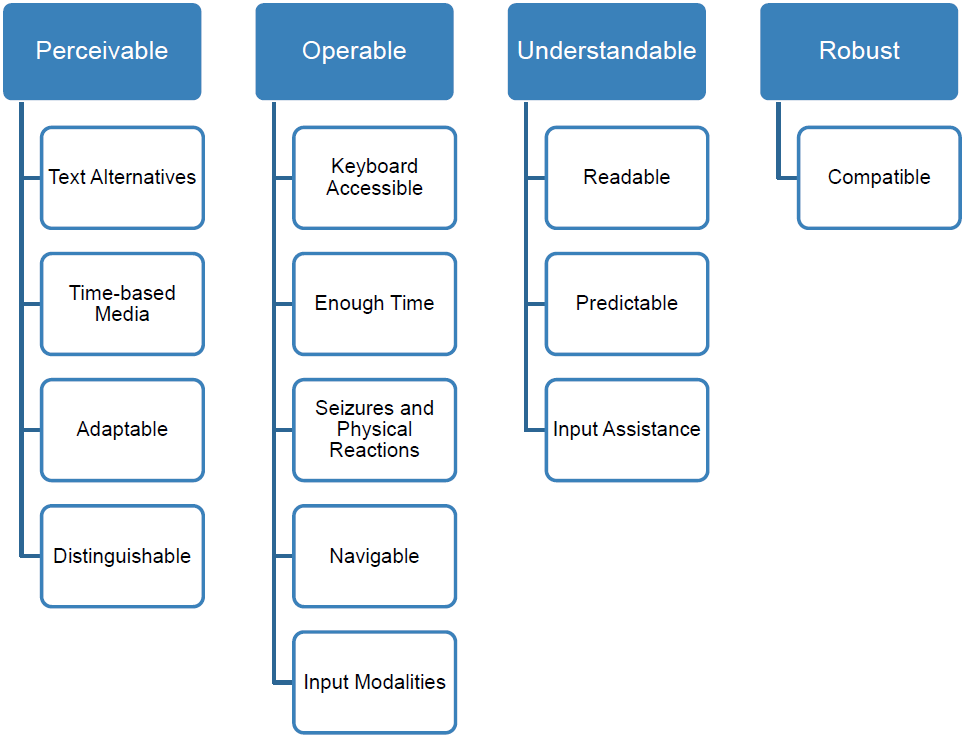
\includegraphics[width=\linewidth]{Images/WCAG_principles_and_guidelines.png}
    \caption{WCAG principles and guidelines}
    \label{fig:wcag_principles_guidelines}
\end{figure}

\chapter{Supporting the Ecosystem: User Agents and Authoring Tools}

For web content to be truly accessible, it is not enough for the content alone to meet standards. The surrounding technology—including the web browsers that display content and the development tools that create it—must also adhere to accessibility principles. The WAI addresses this critical need through two other key specifications: the User Agent Accessibility Guidelines (UAAG) and the Authoring Tool Accessibility Guidelines (ATAG).

\section{User Agent Accessibility Guidelines (UAAG)}

The purpose of UAAG is to provide guidelines for the design of web browsers, media players, and other user agents to ensure they are accessible to people with disabilities. The architecture of UAAG is similar to WCAG, organized around principles and guidelines (See figure ~\ref{fig:uaag_architecture}). The principles for user agents are:

\begin{enumerate}
    \item \textbf{Perceivable:} The user agent must support features that allow users to perceive content, such as providing access to alternative content, highlighting, text and volume configuration, and support for user style sheets.
    \item \textbf{Operable:} The user agent must provide for accessible operation, including full keyboard access, sequential and structural navigation, text search functionality, and support for various input devices.
    \item \textbf{Understandable:} The user agent itself must be understandable and predictable in its behavior. It must provide clear documentation and help users avoid and correct mistakes.
    \item \textbf{Programmatic Access:} This principle, which corresponds to WCAG's "Robust," requires the user agent to support a wide range of assistive technologies. This means browsers must have standard interfaces (APIs) that assistive technologies can use to operate the browser and present content in an appropriate way on behalf of the user.
\end{enumerate}

\begin{figure}
    \centering
    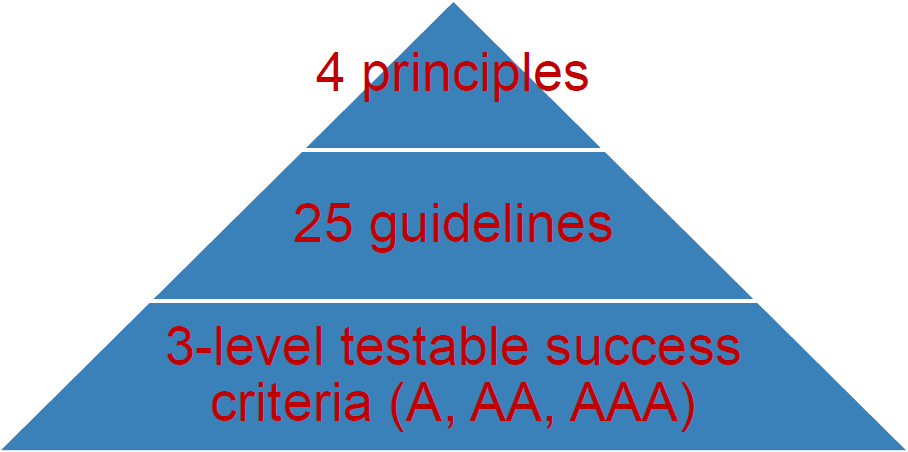
\includegraphics[width=0.5\linewidth]{Images/UAAG_architecture.png}
    \caption{UAAG architecture}
    \label{fig:uaag_architecture}
\end{figure}

\begin{figure}
    \centering
    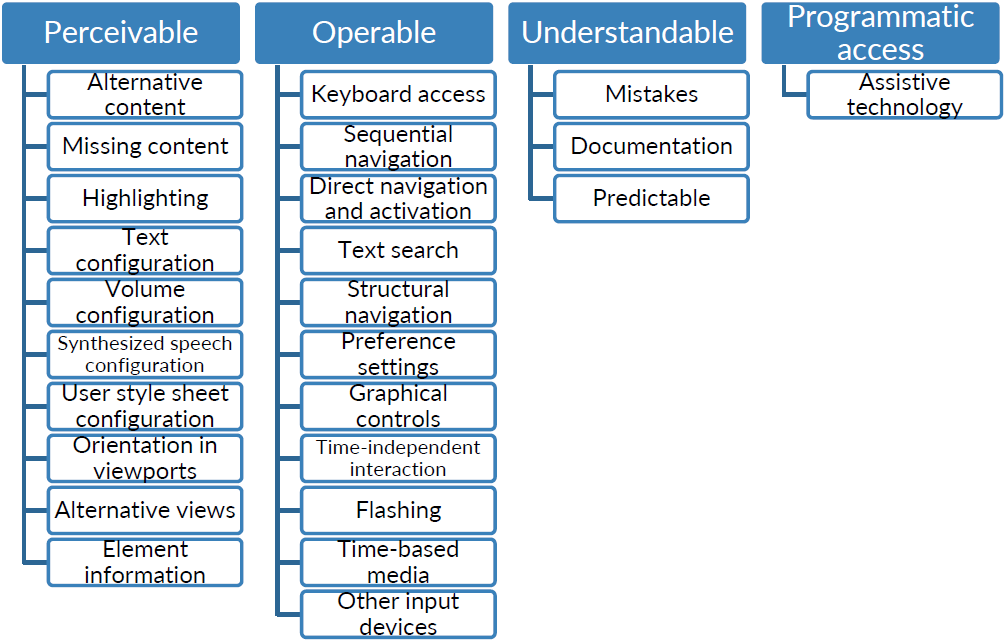
\includegraphics[width=\linewidth]{Images/UAAG_principles_and_guidelines.png}
    \caption{UAAG principles and guidelines}
    \label{fig:uaag_guidelines}
\end{figure}

\section{Authoring Tool Accessibility Guidelines (ATAG)}

ATAG addresses the software and tools that are used to create web content. It plays a crucial dual role in the accessibility ecosystem, which is structured into two main parts:

\subsection{Part A: Make the authoring tool user interface accessible}

This ensures that developers with disabilities can use authoring tools effectively. Its principles require that the tool's user interface and editing views are Perceivable, Operable, and Understandable, with specific guidelines for keyboard access, navigation, and clear documentation.

\subsection{Part B: Support the production of accessible content}

This requires the tool to help all developers—regardless of their own accessibility expertise—create content that conforms to WCAG. The principles for this part are:
\begin{itemize}
    \item \textbf{Automatic processes must produce accessible content:} Any content generated automatically by the tool must be accessible by default.
    \item \textbf{Authors must be supported in creating new accessible content:} The tool should guide authors with features like accessible templates and prompts for alternative text.
    \item \textbf{Authors must be supported in improving existing content:} The tool should be able to identify accessibility problems in existing content and assist the developer in fixing them.
    \item \textbf{Accessibility features must be promoted and integrated:} The tool must document its own accessibility features and make them readily available to authors.
\end{itemize}

Together, these guidelines ensure the entire chain of web production and consumption is accessible. This ecosystem is further enhanced by a specialized standard for today's complex, interactive web applications.

\chapter{Advanced Accessibility for Rich Internet Applications (WAI-ARIA)}

\begin{figure}
    \centering
    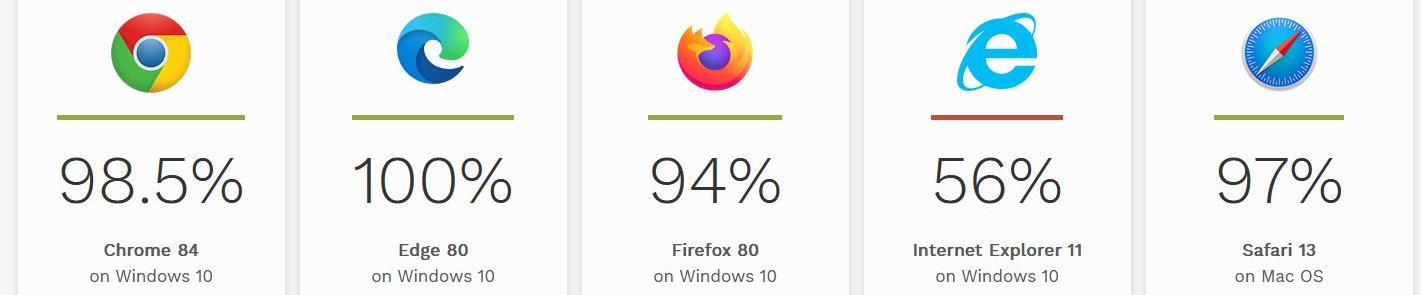
\includegraphics[width=\linewidth]{Images/ARIA_level_of_support.jpg}
    \caption{ARIA level of support by major browsers}
    \label{fig:aria_support}
\end{figure}

The Accessible Rich Internet Applications (WAI-ARIA) suite is a technical specification that addresses the challenges of making modern, dynamic web applications accessible. Unlike the other guidelines, ARIA is not an alternative to WCAG; rather, it is an \textit{orthogonal} specification that works alongside it. It is specifically designed for the dynamic content and advanced user interface controls (widgets, structures, and behaviors) common in rich internet applications. \\

ARIA's approach is semantic. It provides an ontology—a formal vocabulary—that can be added to markup to give assistive technologies more information about the function and state of UI elements. This vocabulary is built on three core concepts:

\begin{itemize}
    \item \textbf{Role:} Defines the type of user interface component (e.g., a "widget" like a slider or a "landmark" like a navigation menu).
    \item \textbf{State:} A dynamic property that expresses the current condition of an object, which may change based on user interaction (e.g., whether a checkbox is checked).
    \item \textbf{Property:} An essential attribute or data value associated with an object that defines its nature (e.g., a property that makes a form field required).
\end{itemize}

ARIA states and properties start with "aria-" and are inserted in the HTML tags as if they were attributes conveying information to assistive technologies. This semantic information allows user agents (browsers) to correctly interpret complex UI components and communicate their role, state, and properties to assistive technologies via a platform \textbf{Accessibility API} (See figure ~\ref{fig:wai-aria_contract_model}). \\

\begin{figure}
    \centering
    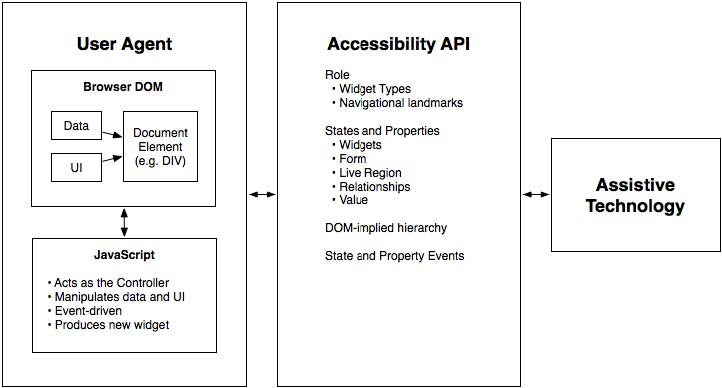
\includegraphics[width=\linewidth]{Images/WAI-ARIA_contract_model.jpg}
    \caption{WAI-ARIA contract model}
    \label{fig:wai-aria_contract_model}
\end{figure}

To ensure seamless integration, the \textbf{HTML Accessibility API Mappings} specification standardizes the connection between the browser's Accessibility API and the native accessibility functions built into major operating systems. This creates a powerful, two-way communication channel. Accessibility features enabled at the operating system level can be reflected in the browser's behavior, and user actions within the browser can be filtered through the OS to interact with devices and assistive technologies correctly. This deep integration maps browser accessibility features to platform-specific APIs like Microsoft's UI Automation, Linux/GNOME's ATK, and Apple's macOS Accessibility Protocol. \\

In conclusion, the W3C's Web Accessibility Initiative provides a comprehensive and interconnected ecosystem of standards. By addressing web content (WCAG), user agents (UAAG), authoring tools (ATAG), and complex applications (ARIA), this framework ensures that all components work together to build a web that is truly accessible to everyone.

\end{document}
